% !TeX root = OptCuts.tex

\section{Results and Discussion}
\label{sec:results}

\subsection{Comparisons}

We demonstrate the capabilities of our framework by comparing to AutoCuts~\cite{Poranne2017Autocuts}, Geometry Images~\cite{Gu2002Geometry}, and Seamster~\cite{Sheffer2002Seamster}.

Since our method can generate UV maps with locally optimal seams under a certain distortion bound, we are able to directly use the output $E_s$ of different methods parameterizating an input surface to the same distortion level as the evaluation metric. This metric is consistent among comparisons with all methods. Moreover, it also fits in well with practical scenarios where the control of distortions are more intuitive to the users and as-short-as-possible seams are expected.

\minchen{[TODO] provide detailed settings on the compared methods, and how much user assistance was needed for other methods}

\paragraph{AutoCuts}
AutoCuts obtains high quality UV maps by involving users into the optimization loop. However, when aiming for convenient, fully-automatic methods, the non-smoothness of their Separation energy not only makes it challenging for global parameter settings, but also often end up the optimization with suboptimal results. To show that we automatically obtain high quality results without suffering these issues, we compare our method with a fully automatic version of AutoCuts obtained under the guidance of AutoCuts authors by constructing appropriate homotopy paths with uniform adaptive parameter settings.

Since AutoCuts does not intuitively support generating UV maps with a certain level of distortion, we first run AutoCuts on a batch of input surfaces, and then set their output distortions as $b_d$ in our method for each input. As demonstrated in Table~\ref{}, we require less time to generate UV maps with not larger distortion and significantly smaller seams. Note that we also enforced bijectivity (Figure~\ref{}), which is only supported in AutoCuts with user assistance on patch manipulation.

\paragraph{Geometry Images}
Geometry Images iteratively finds an extremal point with maximal $L^2$ stretch~\cite{} on the current UV map and make a cut, connecting the extremal point to the current seam with shortest path on the input surface, to reduce distortion on the newly parameterized map. To fairly compare with Geometry Images' cutting strategy, instead of using shape preserving mesh parameterization~\cite{} to always generate a circled UV map, we here change it by minimizing the symmetric Dirichlet energy for parameterization between each cut. Now that our Geometry Images is based on a free-boundary parameterization, the distortion will always decrease after a new cut is introduced, thus we can also set a distortion bound to terminate the algorithm when the bound is reached.

Given the same input surface with our standard UV initialization, we reach identical distortion bounds with shorter seam length (Figure~\ref{fig:comp_GI}). Note that when we asked for more and more isometric UV maps, the quality of the seams by Geometry Images drop drastically while our method keeps generating high-quality seams (See batch comparison statistics in Table~\ref{tb:comp_GI}).

\begin{figure}[!h]
\centering
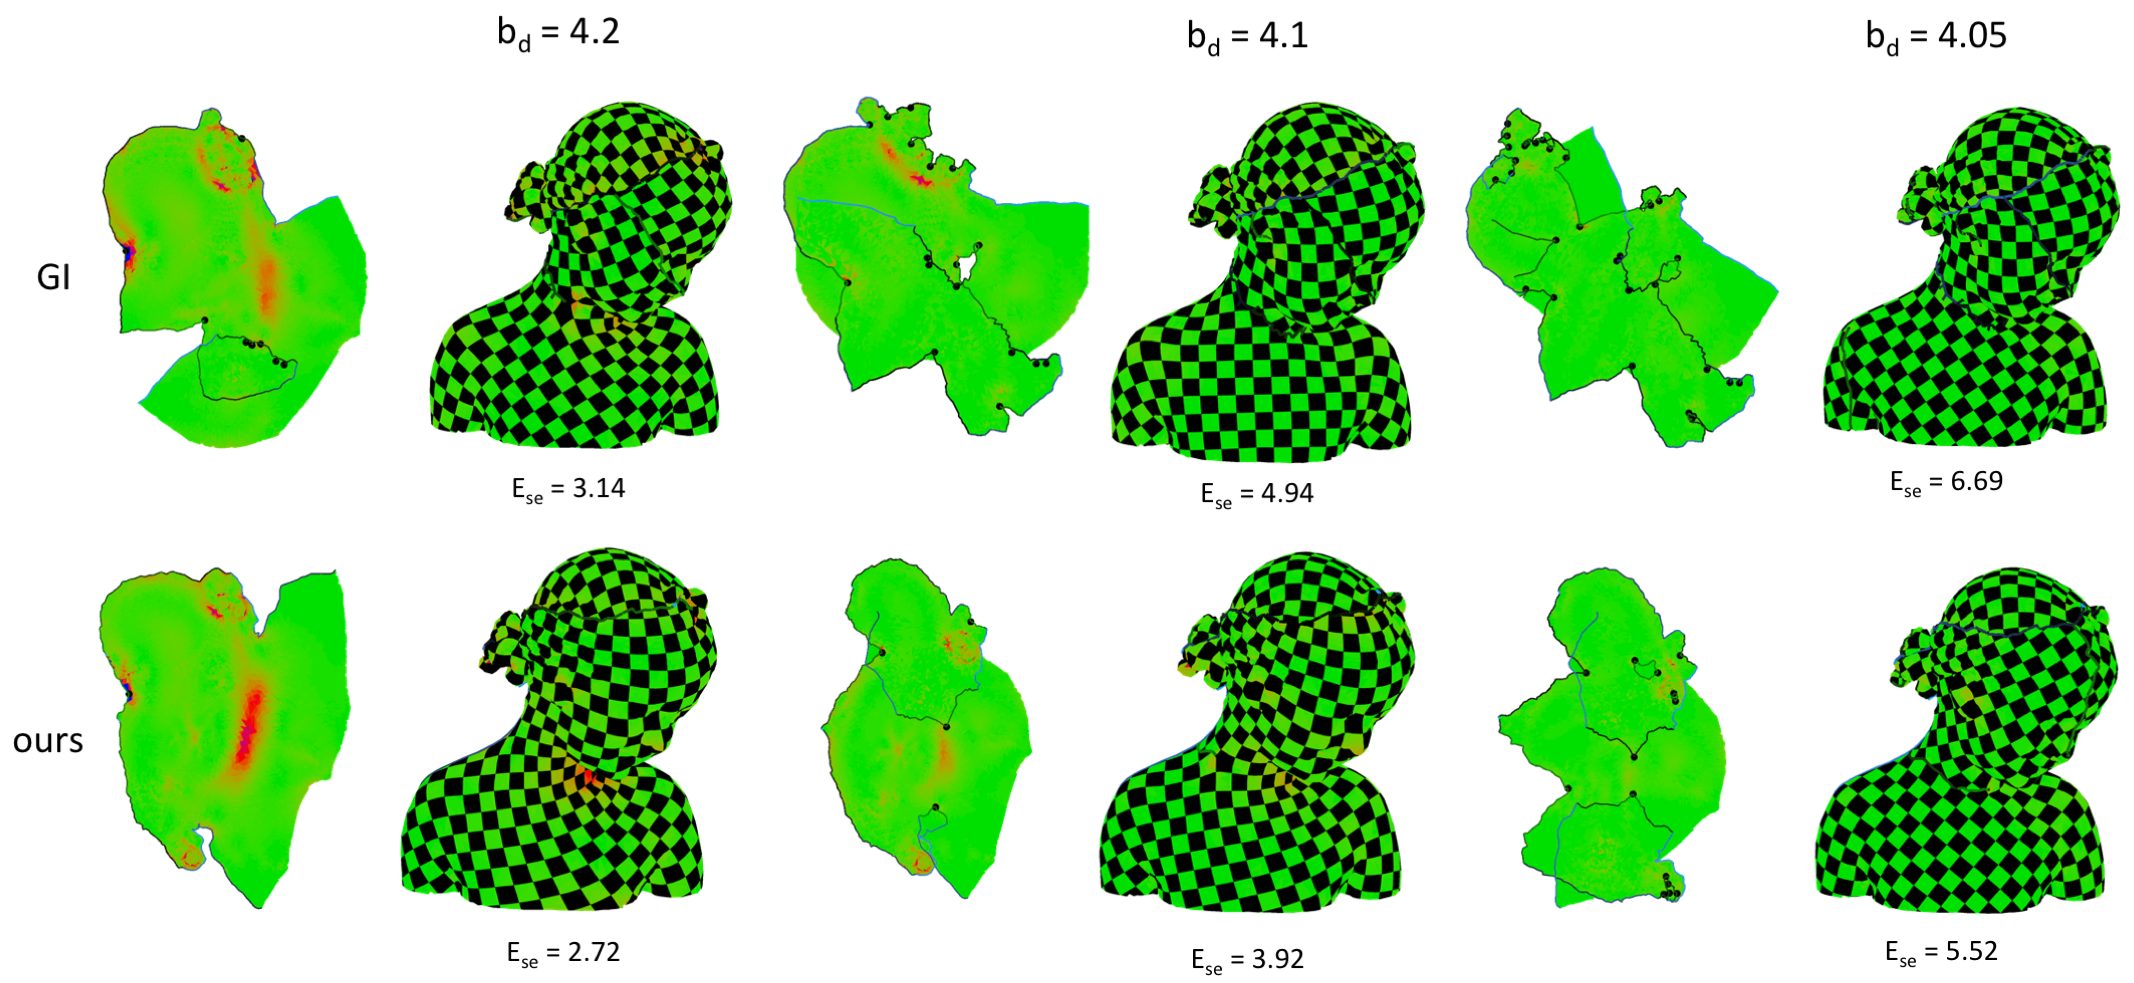
\includegraphics[width=\linewidth]{fig/comp_GI.png}
\caption{Comparison between Geometry Images and our method on the bimba model with $b_d = 4.2, 4.1, 4.05$ from left to right.}
\label{fig:comp_GI}
\end{figure}
% also could be face_f10000, male_body_i_f10000, statue_3_i_f10000, statue_4_i_f10000, statue_5_i_f10000

\begin{table}[!h]
\centering
\caption{Comparisons between Geometry Images and our method on 70 input surfaces with $3721$ vertices per input in average. Two $E_{se}$ are considered to be similar if their ratio lies inside $[0.95, 1.05]$.\minchen{Percentage when our $E_{se}$ is smaller is 58.9\%, 60.3\%, and 64.0\% for $b_d = 4.2, 4.1, 4.05$. Which kind of stats is stronger?} In the last row we start our optimization from the output seams by GI with $b_d = 4.1$ and generates bijective UV maps.} 
\label{tb:comp_GI}
\begin{tabular}{@{}cccccccc@{}}
\toprule
\multirow{2}{*}{$b_d$} & \multicolumn{2}{c}{average $E_{se}$}             & \multicolumn{3}{c}{when our $E_{se}$ is}                         & \multicolumn{2}{c}{average time (s)}       \\ \cmidrule(l){2-8} 
                   & GI & ours & shorter & similar & longer & GI & ours \\ \midrule
4.2                & 4.03             & 3.98           &  47.9\%  & 17.8\%  & 34.2\% & 13.0          & 87.0        \\
4.1                & 4.93             & 4.84           &  43.8\%  & 30.1\%  & 26.0\% & 17.0        & 137.5        \\
4.05               & 6.33             & 6.14           &  45.3\%  & 36.0\%  & 18.7\% &  24.1        & 213.2        \\ 
4.1*               & 4.93             & 4.79           &  48.6\%  & 36.1\%  & 15.3\% &  17.0        & 304.0        \\ \bottomrule
\end{tabular}
\end{table}

If we take Geometry Images output as a fast heuristic initial guess, we can use OptCuts to improve the seam quality towards the locally optimal point while still satisfying the distortion bound. To make this experiment more challenging, we add bijectivity constraints to our framework, which prevents from reaching below the distortion bound with the initial seams. However, we still efficiently obtain bijective UV maps with even shorter seams (Figure~\ref{fig:comp_GI_outputAsInit}, Table~\ref{tb:comp_GI} last row).

\begin{figure}[!h]
\centering
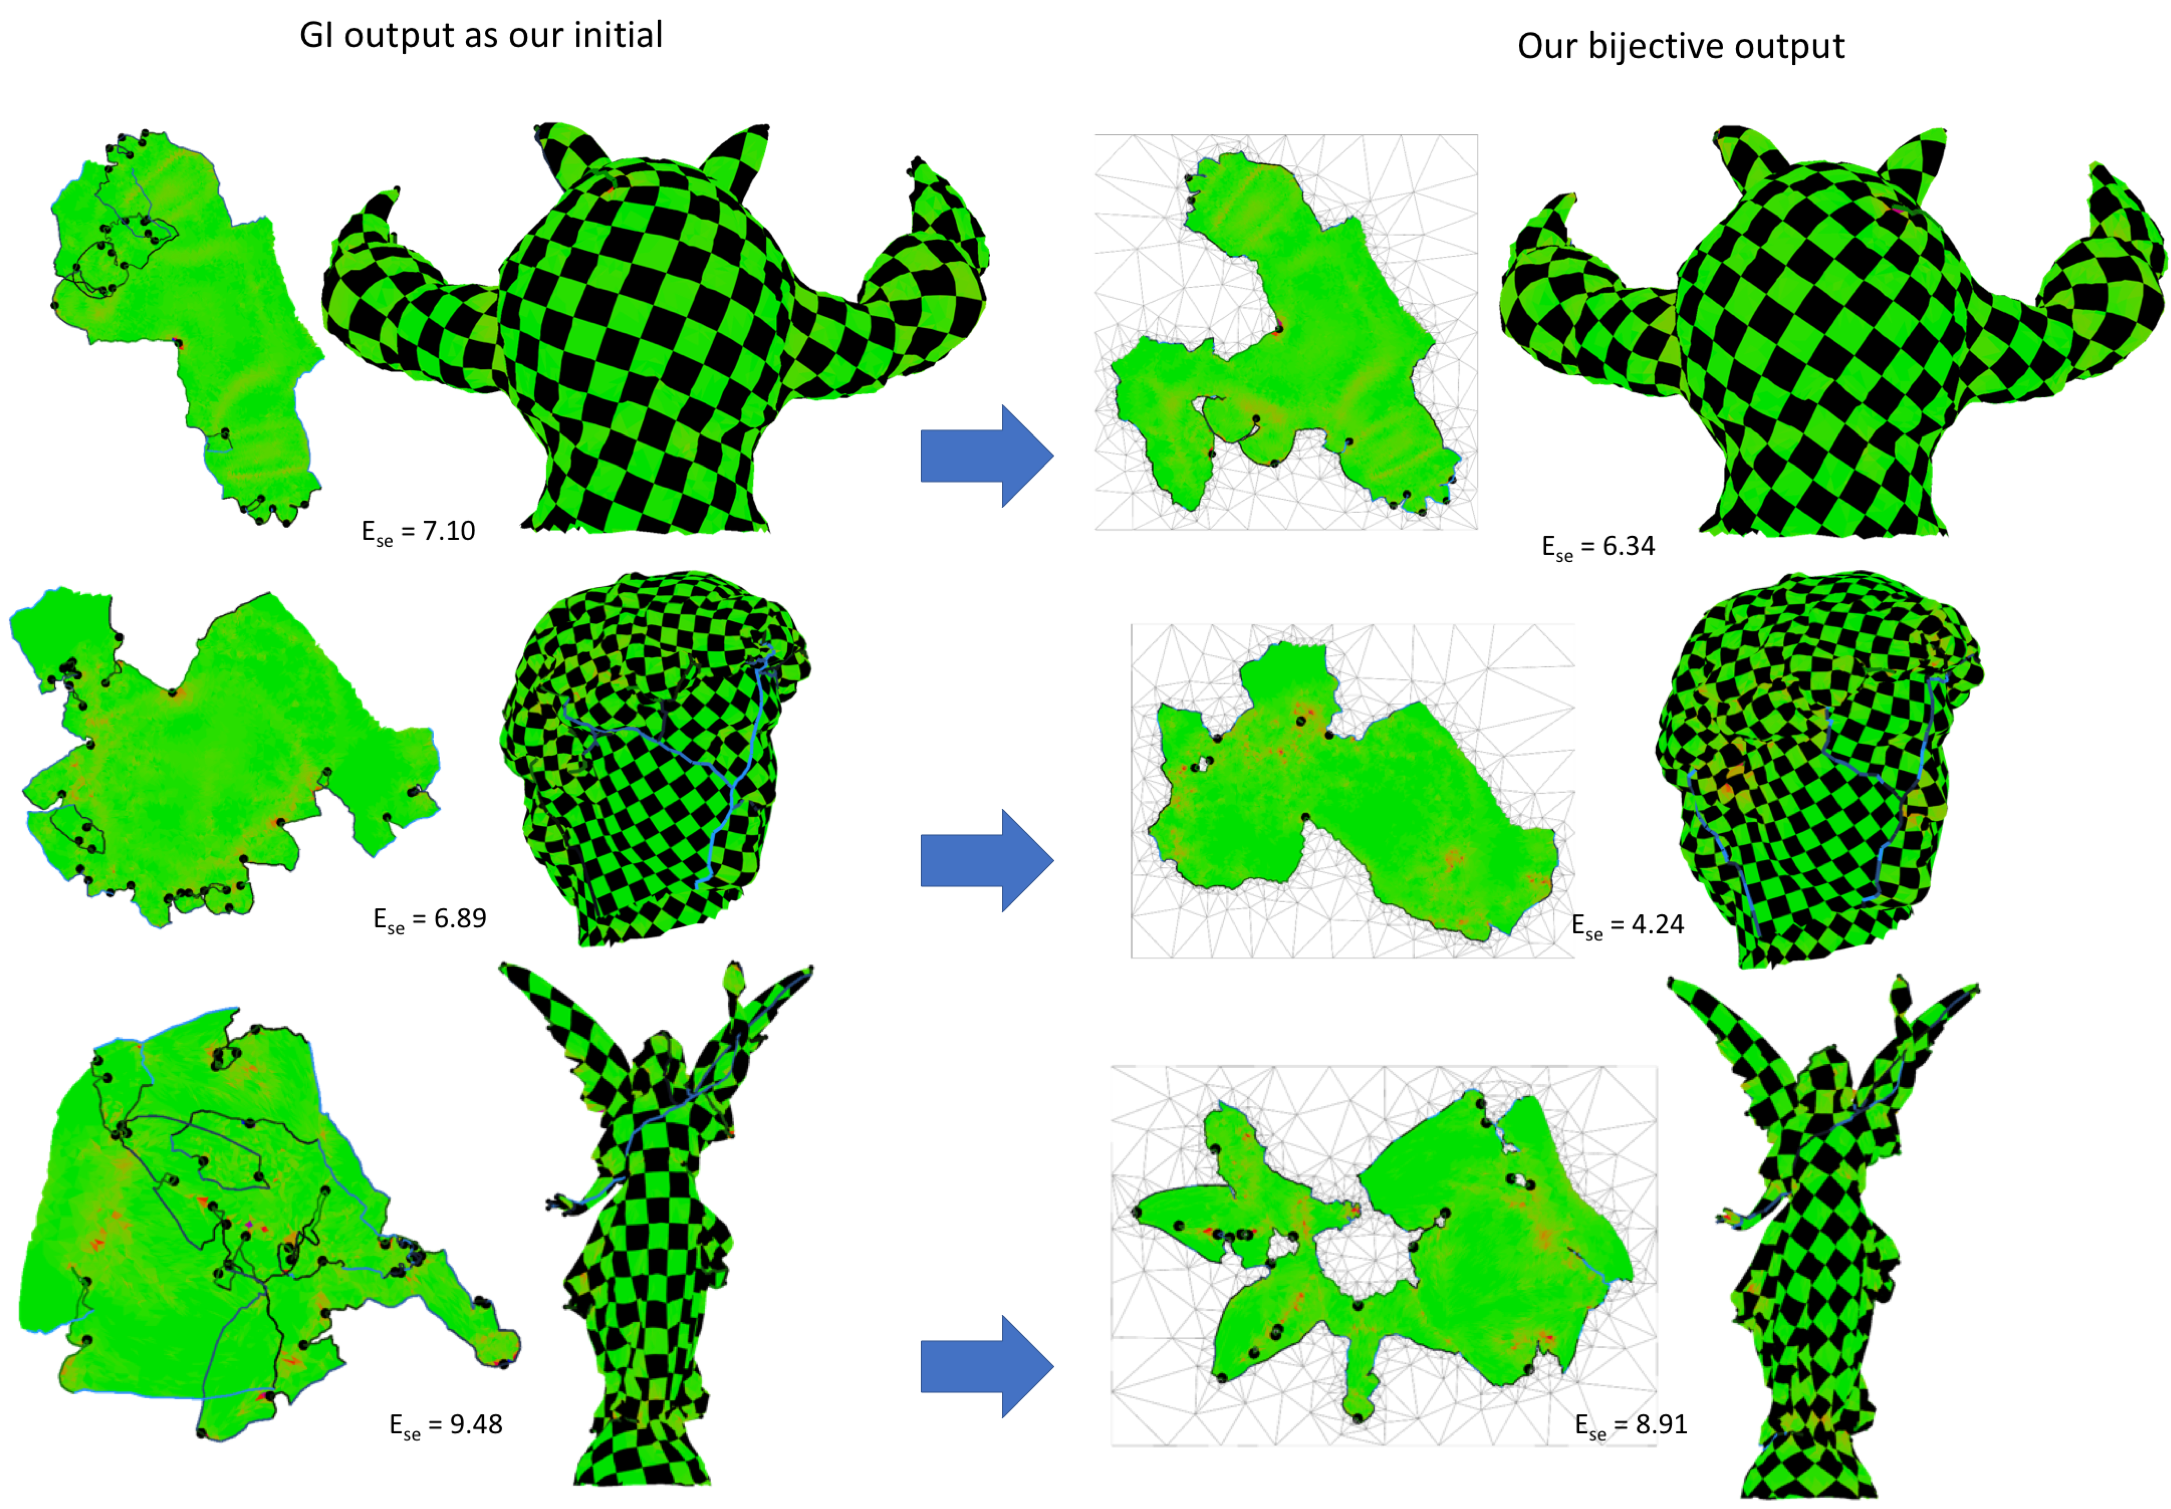
\includegraphics[width=\linewidth]{fig/comp_GI_outputAsInit.png}
\caption{Using Geometry Images output with $b_d = 4.1$ as our initial UV map and distortion bound, we improve seam quality, reaching a locally optimal seam configuration, even with an extra bijectivity constraints.}
\label{fig:comp_GI_outputAsInit}
\end{figure}
% also could be bimba, bunny


\paragraph{Seamster}

\minchen{[TODO] add specific analysis to the comparison between ours and the 3 methods}

They key difference between our framework and two-pass methods is that, our seams are computed to directly improve the given distortion measure rather than some approximated heuristics. Besides, since the problem is highly nonlinear, seams that benefits one region might be redundant due to the existance of another seam in a near or far region. Our framework is capable of removing those redundancy with our topology search, but the two-pass methods can not.


\subsection{Experiments}
\label{sec:results_exp}

\paragraph{Initial Embedding}
To show that we search for locally optimal UV maps regardless of the given initial embedding, we run our method starting from our standard initializations, triangle soups, and preliminary UV maps produced by other methods or by the users. All the output UV maps are with high quality (Figure~\ref{fig:bad_init_still_ends_well}) \minchen{[TODO]}.

\paragraph{Triangulation Invariance} \minchen{[TODO] not sure whether applicable}

\paragraph{Scalability} \minchen{[TODO]}

\subsection{Variations}
\label{sec:results_variations}

Without changing the framework, simply reformulating $L = E_s + \lambda E_d$ according to different needs enables OptCuts to solve mesh parameterization problems in many variations:

\paragraph{Global Bijectivity} \danny{suggest we no longer consider this a variation and instead use it as a key part of our full algorithm - see my comments earlier.} \minchen{[DOING]} Augmenting our $E_d$ with a collision handling energy $E_b$ will easily achieve joint seam placement and bijective mesh parameterization. We show that by adding a scaffold mesh~\cite{Jiang2017Simplicial} to the voided regions of the UV map and preventing the scaffold mesh from degenerate, our method automatically generate high-quality bijective maps with optimal seams different from that of locally injective parameterization (Figure~\ref{fig:bijective_vs_injective}). When computing $\hat{f}_e$, besides also including the one-ring triangles on the scaffold mesh for computing energy decrease, we also need to move the splitted vertices slightly apart to leave room for inserting new scaffold mesh triangles.

\paragraph{Conformal Parameterization} \minchen{[TODO]} Using a conformal energy~\cite{Hormann2000MIPS,Sheffer2005ABFPP} for $E_d$ will achieve joint seam placement and conformal parameterization. Figure~\ref{fig:conformal_vs_isometry} shows some results with $E_d = E_{ABForMIPS}$~\cite{} compared to results with $E_d = E_{SD}$, where different seams are generated while our framework stays the same.

\paragraph{Regional Seam Placement} \minchen{[TODO]} On the discrete side, if we reweight $E_{SL}$ with an edge prior provided by the user or an algorithm~\cite{} as
\[ E_s = \hat{E}_{SL} = \sum_{i\in\mathcal{S}} w_{SL,i} E_{SL,i} \quad w_{SL,i} \in \mathcal{R^+} \]
we could bias the seam placement towards regions e.g. where continuity is less in demand (Figure~\ref{fig:regional_seam_placement}).

\minchen{[TODO] add specific analysis to the results}

The key is that with all these variations, our framework stays the same, and it efficiently generates optimal seams for the specific problem formulation.